Eine Bewegung wird durch das $s(t)$-Diagramm links beschrieben. Welches der beiden $v(t)$-Diagramme (1) und (2) beschreibt die gleiche Bewegung? Zeichnen Sie das $s(t)$-Diagramm zum anderen $v(t)$-Diagramm.

\begin{center}
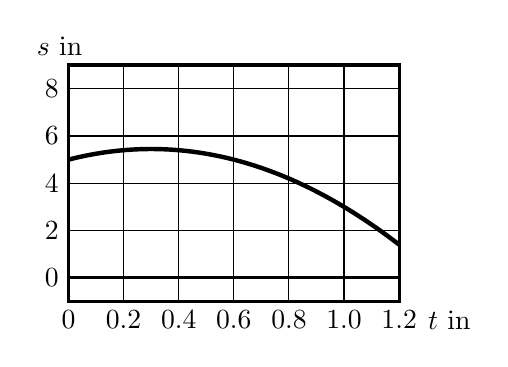
\begin{tikzpicture}[>=stealth, xscale=3.5, yscale=0.3]
 \foreach \x in {0.2,0.4,0.6,0.8,1.0} \draw (\x,-1) -- (\x,9);
 \foreach \y in {0,2,4,6,8} \draw (0,\y) -- (1.2,\y);
 \draw[very thick] (0,0) -- (1.2,0);
 \draw[very thick] (0,-1) rectangle (1.2,9);
 \foreach \x in {0,0.2,0.4,0.6,0.8,1.0,1.2} \node[below] at (\x,-1) {\x};
 \foreach \y in {0,2,4,6,8} \node[left] at (0,\y) {\y};
 \node[anchor=north west] at (1.27,-1) {$t$ in \si{\second}};
 \node[above right] at (-0.15,9) {$s$ in \si{\meter}};
 \draw[ultra thick, domain=0:1.2, samples=60] plot (\x, {5+3*\x-5*\x*\x});
\end{tikzpicture}
\hspace{6mm}
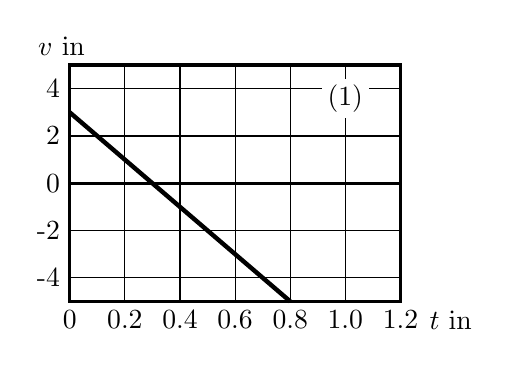
\begin{tikzpicture}[>=stealth, xscale=3.5, yscale=0.3]
 \foreach \x in {0.2,0.4,0.6,0.8,1.0} \draw (\x,-5) -- (\x,5);
 \foreach \y in {-4,-2,0,2,4} \draw (0,\y) -- (1.2,\y);
 \draw[very thick] (0,0) -- (1.2,0);
 \draw[very thick] (0,-5) rectangle (1.2,5);
 \foreach \x in {0,0.2,0.4,0.6,0.8,1.0,1.2} \node[below] at (\x,-5) {\x};
 \foreach \y in {-4,-2,0,2,4} \node[left] at (0,\y) {\y};
 \node[anchor=north west] at (1.27,-5) {$t$ in \si{\second}};
 \node[above right] at (-0.15,5) {$v$ in \si{\meter\per\second}};
 \draw[ultra thick] (0,3) -- (0.8,-5);
 \node[fill=white, inner sep=2pt] at (1.0,3.6) {(1)};
\end{tikzpicture}
\hspace{6mm}
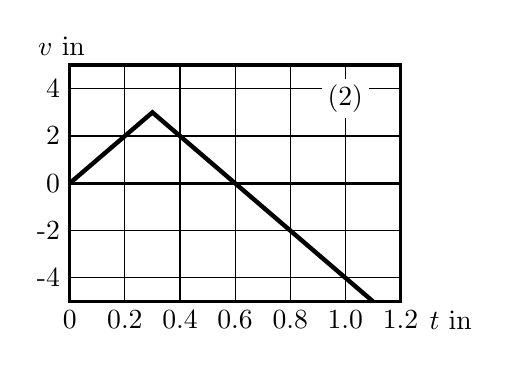
\begin{tikzpicture}[>=stealth, xscale=3.5, yscale=0.3]
 \foreach \x in {0.2,0.4,0.6,0.8,1.0} \draw (\x,-5) -- (\x,5);
 \foreach \y in {-4,-2,0,2,4} \draw (0,\y) -- (1.2,\y);
 \draw[very thick] (0,0) -- (1.2,0);
 \draw[very thick] (0,-5) rectangle (1.2,5);
 \foreach \x in {0,0.2,0.4,0.6,0.8,1.0,1.2} \node[below] at (\x,-5) {\x};
 \foreach \y in {-4,-2,0,2,4} \node[left] at (0,\y) {\y};
 \node[anchor=north west] at (1.27,-5) {$t$ in \si{\second}};
 \node[above right] at (-0.15,5) {$v$ in \si{\meter\per\second}};
 \draw[ultra thick] (0,0) -- (0.3,3) -- (1.1,-5);
 \node[fill=white, inner sep=2pt] at (1.0,3.6) {(2)};
\end{tikzpicture}
\end{center}
